\documentclass{sig-semester}

\pdfpageheight=11in
\pdfpagewidth=8.5in

\usepackage{latexsym}
\usepackage{amsmath}
\usepackage{amssymb}
\usepackage{color}
\usepackage{enumerate}
\usepackage{graphicx}
\usepackage{amssymb}
\usepackage{epstopdf}
\usepackage{xspace}

% These are from candidacy edic.tex
\graphicspath{{./graphics/}}
\DeclareGraphicsExtensions{.pdf,.jpeg,.png}

% Legacy from Christoph's paper:
% \DeclareGraphicsRule{.tif}{png}{.png}{`convert #1 `dirname #1`/`basename #1 .tif`.png}

% When converting eps to pdf, suffix is added to filename. 
% Recommended not to be empty string by http://www.tex.ac.uk/tex-archive/macros/latex/contrib/oberdiek/epstopdf.pdf : page 4, suffix paragraph.
\epstopdfsetup{suffix=-generated}


\newtheorem{theorem}{Theorem}[section]
\newtheorem{proposition}[theorem]{Proposition}
\newtheorem{example}[theorem]{Example}
\newtheorem{remark}[theorem]{Remark}
\newtheorem{todo}[theorem]{ToDo}
\newtheorem{algorithm}[theorem]{Algorithm}
\newtheorem{metatheorem}{Metatheorem}[section]
\newtheorem{definition}[theorem]{Definition}
\newtheorem{property}[theorem]{Property}
\newtheorem{corollary}[theorem]{Corollary}
\newtheorem{lemma}[theorem]{Lemma}
\newtheorem{conjecture}[theorem]{Conjecture}
\newtheorem{proviso}[theorem]{Proviso}

\newcommand{\tuple}[1]{{\langle#1\rangle}}


\title{Experiments for Parallelizing of Large Scale Databases}


%\numberofauthors{1}
\author{\alignauthor Aleksandar Vitorovic \\[1ex]
\affaddr{Dept.\ of Computer Science} \\
\affaddr{EPFL} \\
\affaddr{aleksandar.vitorovic@epfl.ch}
}

\def\SQL{SQL\xspace}
\def\OLAP{OLAP\xspace}
\def\OLTP{OLTP\xspace}
\def\M3{M3\xspace}
\def\EXORD{actual trigger execution order\xspace}

\begin{document}
\maketitle


\abstract{
This paper presents issues related to experiments and more insight view of the system.\\
}


\keywords{Incremental View Maintenance, \OLAP updates, Parallelization, Expreriments}


\section{Introduction}
\vspace{2mm}

\subsection{Restricted M3}

For the purposes of this paper, we restrict ourselves to a limited, fully incremental version of \M3.
\begin{itemize}
\item \textit{All loop variables appear on both sides of a statement.} A loop variable is a variable not existing in the trigger arguments. The natural implication of a loop variable appearing only on the right-hand side is as a sum aggregate over the variable. In restricted M3, this aggregate can be computed incrementally by maintaining an additional map with one fewer key.
\item \textit{All loop variables appear as a parameter to exactly one right-hand side map.} A loop variable that appears in two right-hand side maps is effectively a join between the maps.  In restricted M3, joins are computed incrementally using event variables. Note that this restriction results in each loop variable's domain being defined by exactly one map.
\item \textit{Terms do not contain conditions.} Unrestricted M3 supports conditioned non-incremental aggregates.
\item \textit{Map data dependencies are acyclic, even across multiple events.} A non-recursive SQL query may be represented as an M3 program with no cyclic data dependencies. Restricted M3 does not attempt to support recursive queries.
\end{itemize}

There is no nested queries and binding propagation, only equijoins. Only COUNT, AVG and SUM aggregate joins are supported, while MAX and MIN are not. This is due to fact that for running MAX/MIN joins the system requires huge additional data structures such as sorted list of all values inserted until now.

* no the right-hand side IfElse block,   
* MapAccesses do not have input variables, such as q[``a``][], only output variables, such as q[][''a``]. Copied from Oliver's mail: ''Input variables are variables for which the domain (variable values that we're interested in) is not known until the map is accessed.  Consequently, the best we can do is cache the values we've seen so far and maintain a corresponding output map for each.  This essentially means that we need to rerun the entire query from scratch every time we see a new value.`` From sigmod10-spread: ''However, we never need to do this if all the joins in the query are equijoins. `` 

Inequalities are possible only with constants (there are some others supported as well, but it is hard to define which one is supported). Practically, if they form bigsum structure, we will loose bounded-in feature for Source-Computation-Destination, and thus data-parallel property is loosed. Theoretical foundations for this can be found in Koch's PODS 2010 paper.

\section{Task 1 - Printings}
\vspace{2mm}

\subsection{Slices explanation.}
\textbf{Next part of text is copied from cidr11-dbtoaster.tex (DBToaster: Agile Views in a Dynamic Data Management System):}

\begin{verbatim}
on_insert_customer(ck,nm,nk,bal):
  m[][ordkey,sprior] += m_c[][ck,ordkey,sprior];
\end{verbatim}

Above, we have a trigger statement in a C-style language firing on insertions to
the {\tt Customer} relation, describing the maintainence of $m$ by reading the
entry $m_c[\mbox{{\tt ck}},ordkey,sprior]$ instead of evaluating $q_c(\mbox{{\tt
ck}}, Orders, Lineitem)$. Notice that the trigger arguments do not contain
$ordkey$ or $sprior$, so where are these variables defined? In DBToaster, this
statement implicitly performs an iteration over the domain of the map being
updated. That is, map $m$ is updated by looping over all $\tuple{ordkey,sprior}$
entries in its domain, invoking lookups on $m_c$ for each entry and the trigger
argument {\tt ck}. Map read and write locations are often (and for a large class
of queries, always) in one-to-one correspondence, allowing for an embarrassingly
parallel implementation. For clarity, the verbose form of the statement is:

\begin{verbatim}
on_insert_customer(ck,nm,nk,bal):
  for each ordkey,sprior in m:
    m[][ordkey,sprior] += m_c[][ck,ordkey,sprior];
\end{verbatim}

\noindent Throughout this document we use the implicit loop form.
Furthermore, this statement is never implemented as a loop, but relies on a map
data structure supporting partial key access, or \textit{slicing}. This is
trivially implemented with secondary indexes for each partial access present in
any maintenance statement, in this case a secondary index yielding all
$\tuple{ordkey,sprior}$ pairs for a given \texttt{ck}.
This form of maintenance statement is similar in structure to the concept of
\textit{marginalization} in probability distributions, essentially the map $m$
is a marginalization of map $m_c$ over the attribute \texttt{ck}, for each
\texttt{ck} seen on the update stream.

\textbf{End of copied section.}

\textbf{Next part is copied from pvldb11-Cumulus (Cumulus: Combining Periodic and Eventual Consistency (in the cloud)):}

\begin{example}
Consider the following M3 statement with maps \texttt{m1} and \texttt{m5}, each partitioned only on attribute N.
\begin{verbatim}
ON +ORDERS(C,O,D) DO { m1[O,N] += D * m5[C,N] }
\end{verbatim}
When event \texttt{+ORDERS} occurs, each node storing a segment of \texttt{m5} will send each value in its segment to the node storing the corresponding segment of \texttt{m1}. If the partition boundaries of \texttt{m1} and \texttt{m5} are identical, each \texttt{m5} node will send its entire segment to exactly one \texttt{m1} node. Note that If the same node stores each pair of corresponding \texttt{m1} and \texttt{m5} partitions, no actual data transmission occurs.  
\end{example}

Even if \texttt{m5} is also partitioned over \texttt{O}, each \texttt{+ORDERS} event updates only one map segment per \texttt{B} value; A node storing a segment of \texttt{m5} is still only required to send the segment to one \texttt{m1} node.  However, there are situations where multicast is required.  

\begin{example}
Consider the following statement:
\begin{verbatim}
ON +ORDERS(C,O,D) DO { q[P,N] += D * m4[O,P] 
                                   * m5[C,N] }
\end{verbatim}

Let \texttt{q} have 10 partitions in a grid pattern, with the domain of \texttt{P} split in half and \texttt{N} split into 5 parts.  Let \texttt{m4} and \texttt{m5} use the same partitioning scheme (with 2 and 5 partitions, respectively). In this instance, when an \texttt{ORDERS} event occurs, each \texttt{m4} node sends its segment to each of the corresponding 5 \texttt{q} nodes, while each \texttt{m5} node will send its segment to each of the corresponding 2 \texttt{q} nodes. 

If a right-hand side map contains an event variable, only a subset, or slice of the map is sent.  For example:
\begin{verbatim}
ON +ORDERS(C,O,D) DO { m1[O,N] += D * m5[C,N] }
\end{verbatim}
In this instance, only the slice \texttt{m5'[N] = m5[C,N]} is sent.
\end{example}

\textbf{End of copied section.}

\textbf{Copied from cumulus/docs/implementation.txt:}

In order to streamline the process of evaluating updates, each node performs some precomputation to figure out where it needs to send data, and where it expects to receive data from, given a particular update.  For each template, at each node, we compute an n-dimensional grid, one dimension for each variable/parameter in the template's input relation.  The domain of each dimension is the least common multiple of the number of partitions across the variable in each MapEntry in the template it appears in.

  eg: Consider the template: ON MYRELATION(Foo) Map 1[Foo, Bar] += Map 2[Foo] * Map 3[Bar];
  In our layout, Map 1 has a 2x2 partitioning scheme, while Map 2 has 4 partitions.  For this template and 
  layout, we would use a 1-dimensional grid of size 4 (LCM of 2 and 4).  If Map 2 had 5 partitions, we would 
  use a 1-dimensional grid of size 10 (LCM of 2 and 5).  However, because we use powers of 2 for our 
  partitioning, the LCM is always the MAX number of partitions over that variable.

\textbf{End of copied section. }

\subsection{Our solution - the messages code.}
In order to understand the rest of the system, partitioning map collections has to be explained. Map collection has a name and it is partitioned among one or more dimensions. Each dimension have specified size, and all the possible key values on a dimension (infinite domain) have to be spreaded among finite (dimension\_size) domain. A unique combination of values from each dimension's finite domain constitutes a map partition. The partition is a unit of storing maps on nodes. All the maps from a single partition belongs to the same node. For the simplicity reasons, the mapping from key values to partitions is done by moduo function.

The goal of this code is to convert parsed M3 statements and trigger instantiation arguments in the form of OCaml expressions into a set of PUT, FETCH and PUSH messages between partitions (or DW Nodes). Map collections, loop variables and aggregate sums (bigsum) are properly recognized and processed. Although lhs maps assigns values from the rhs maps sharing the same key on the same variable, situation with partitions may complicate things a bit. The maps on the lhs and rhs sharing the same map, must have the same number of dimensions, but the appropriate dimension sizes may differ. In a case of simple m1[A]=m2[A] statement, where A is a loop variable, depending on partitioning, single m2 map could participate in multiple m1 map computations, or multiple m1 maps could take part in a single right-hand side computation. Since our approach is moduo based, the messages are sent to appropriate partitions in the round-robin manner.

A user may also be interested in all the possible messages between partitions without knowing trigger instantiation arguments in advance. Our system is also capable of enumerating all the arguments which may create different messages on the output, and for each of them, create that output. This is especially useful when a DW Node is interested at compile time which other nodes it may communicate with.

\subsection{Limitations.}
\begin{enumerate}
 \item Partitioning scheme from files. Using cumulus/data/tpch\_PPSS.sql or cumulus/data/switch\_test\_1.unit. Using parsing from (1) Oliver tutorial section 12 or (2) util/DTDBebug.ml
 \item Only int is supported as type of input/output variables in MapAccess.
 \item For each map access one message is generated (various optimizations could be applied, as explained in semesterPaper)

 \item For now we suppose all partitions are powers of 2, so max is taken. Otherwise LCM should be taken.
 \item Check whether non-trigarg variable is on both sides max once! I said max because BigSum is supported as well, allowing some loop variables to appear only on the rhs.
\end{enumerate}

\section{Task2 - Storage Layer }
\vspace{2mm}
For each Log structure, separate storage structure is implemented.

\subsection{WriteStorage.} 
UML diagram for WriteStorage is presented in Figure~\ref{fig:writeStorage}.

\begin{figure*}
\centering
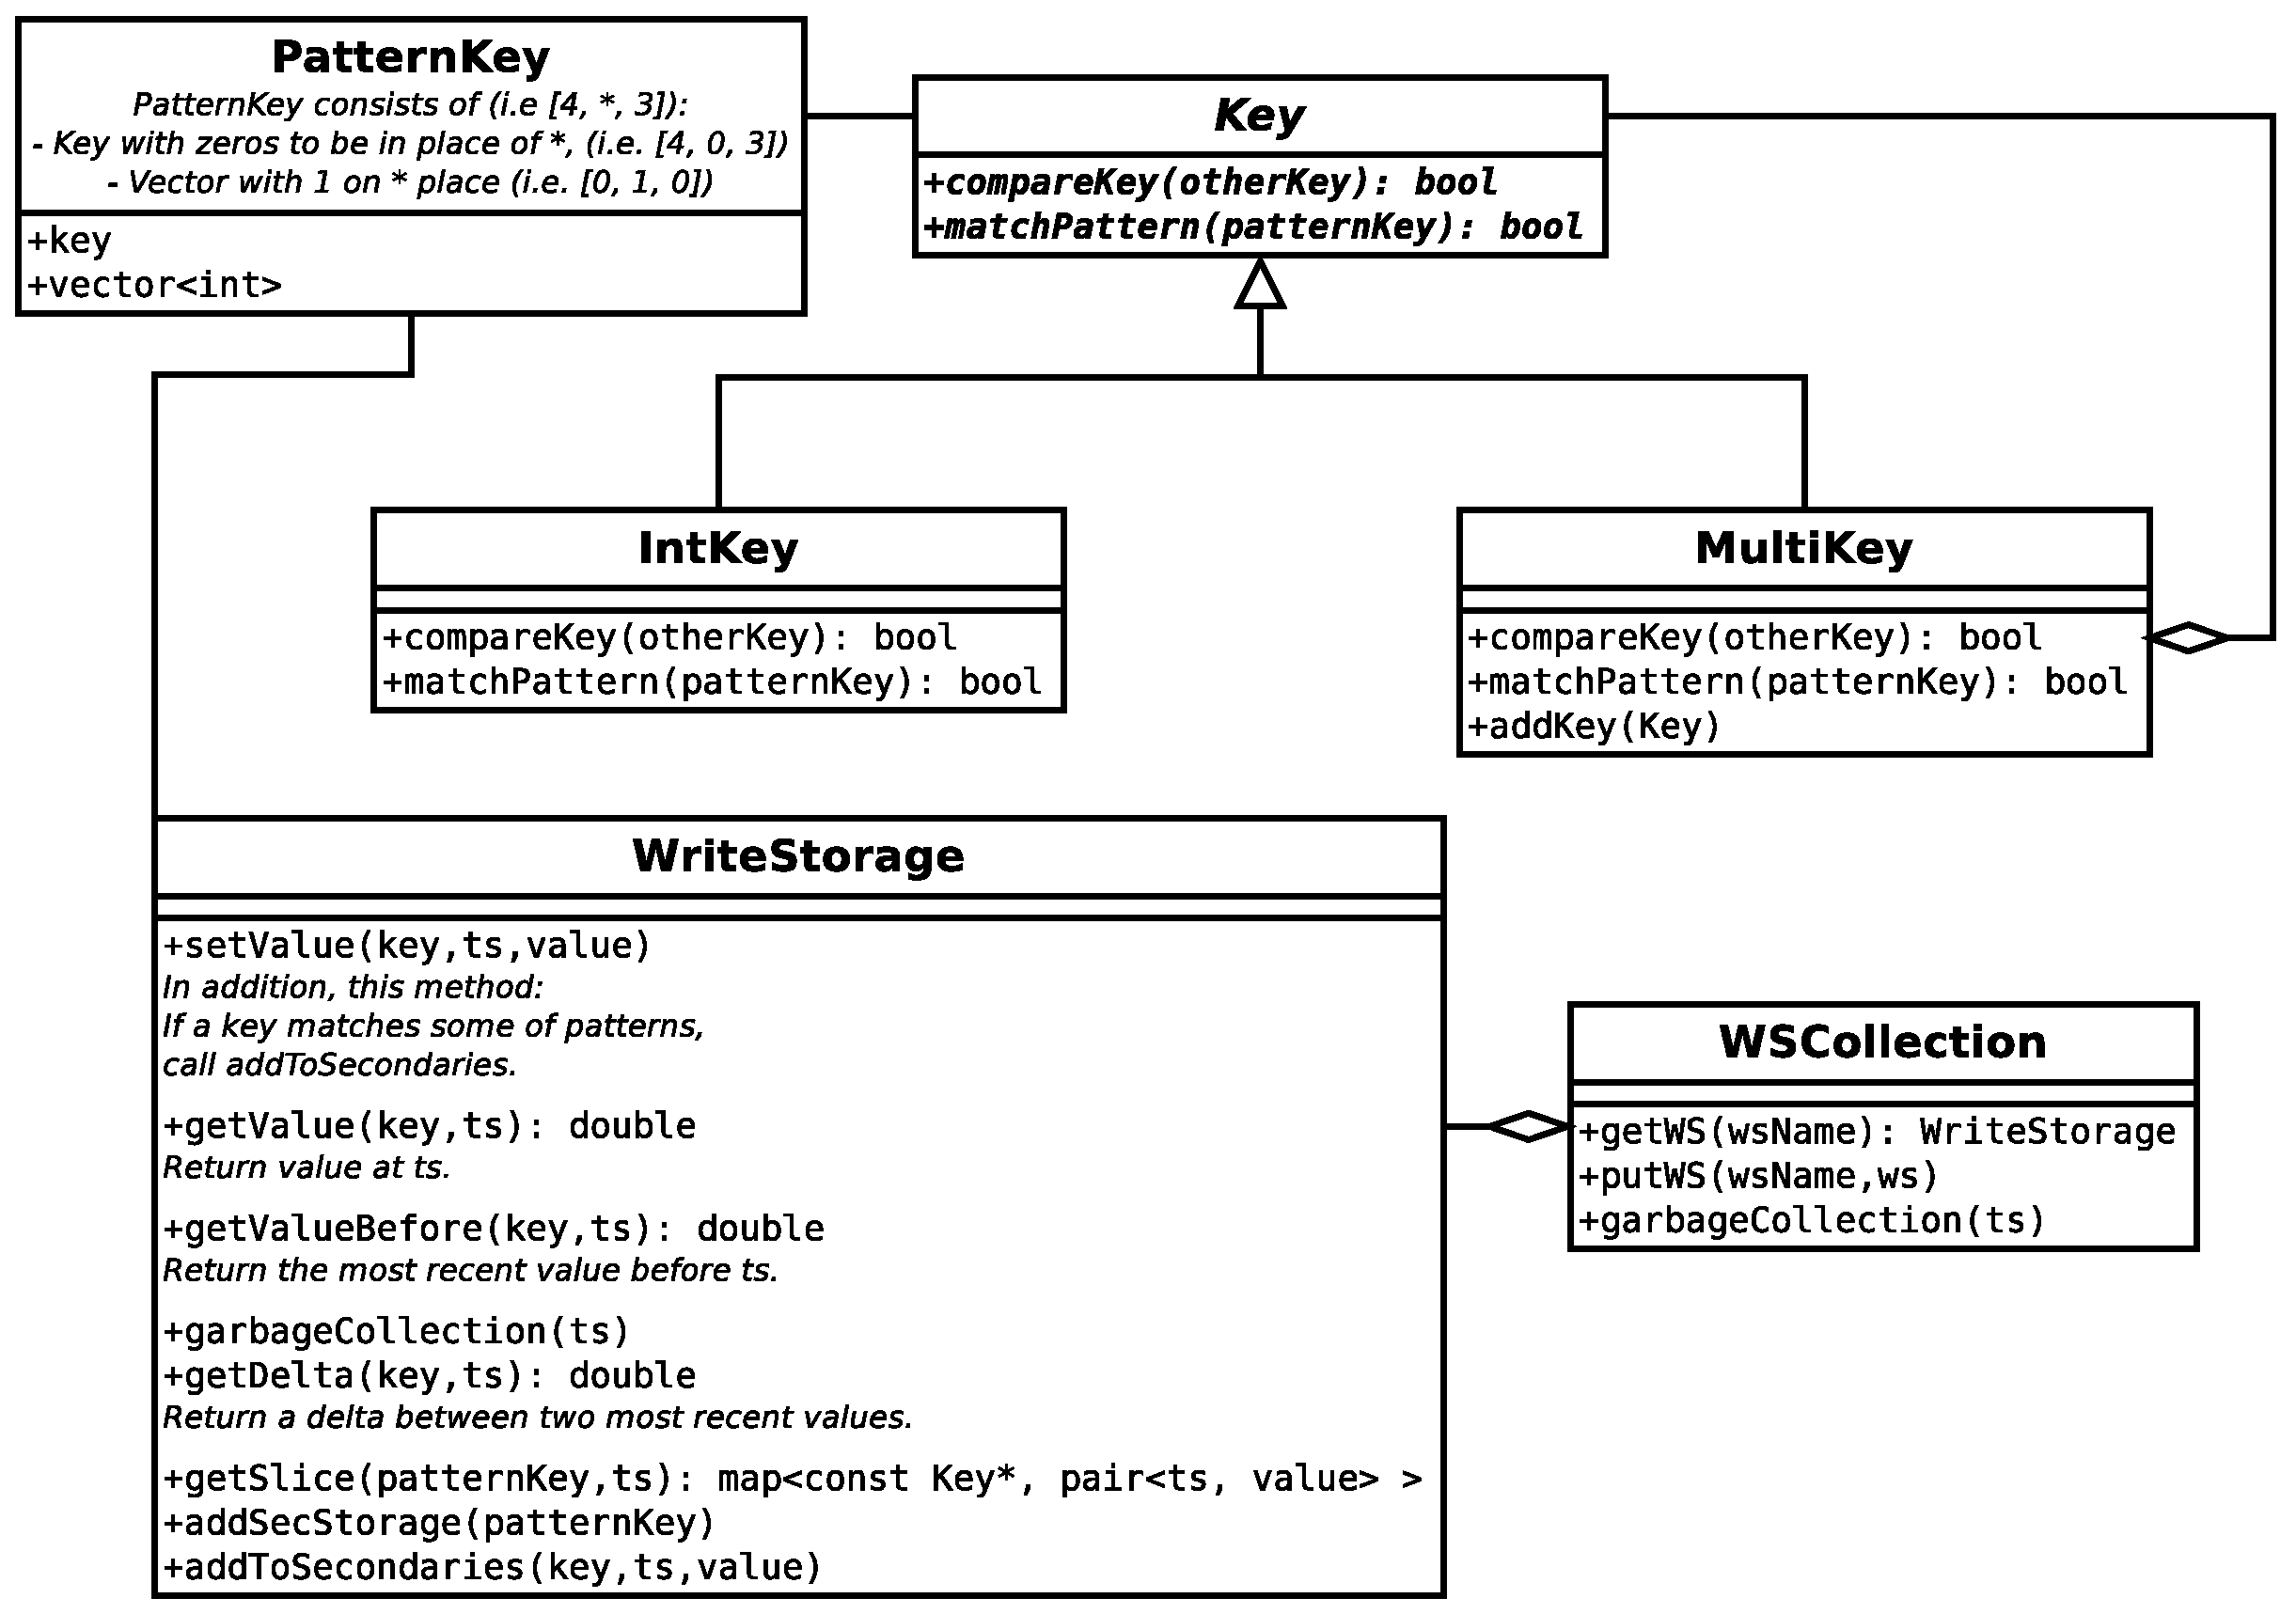
\includegraphics[width=6in]{WriteStorage.eps}
\vspace{-3mm}
\caption{WriteStorage implementation.}
\label{fig:writeStorage}
\vspace{-2mm}
\end{figure*}

Since types and number of dimensions vary, an efficient solution for storing map collections is necessary. Templates programming in these case seems much more complex than applying Composite design pattern on classes Key, IntKey and MultiKey.

The basic data structure for WriteLog is the STL \\ unordered\_map. The key is MultiKey from Figure~\ref{fig:writeStorage}, consisting of possibly multiply keys of different types, depending on partitioning. The value is another data structure with <ts, value> pairs. Due to out-of-order arrival of trigger instantiations, map values at each timestamp have to be checked on read. If these pairs are sorted, the structure will be optimized for reads and garbageCollection, but not for write. Since read operation is more frequent than write (for one lhs there may be multiple rhs), STL:map is used for representing these pairs with TS as sorting parameter. (In STL:map, Less<obj> is the only necessary operation, while == is automatically generated as !(a<b || b<a)).

C++ STL is the hash key/value store implementation used in Cumulus. Berkeley DB offers the same functionality through different method name, and in addition can store excessive data on disk.

WriteStorage embodies this data structure with necessary methods, representing a map collection. Map name is not stored here, but rather in WSCollection, as the way for differentiation of all the map collections on the DW Node.

\textbf{Secondaries.} GetSlice method allows for acquiring multiple maps at a time. For example if map collection m1 has 4 dimensions, m1[*,*,*,*] and m1[4,2,*,7] are valid accesses. First one returns whole map collection (maps are not sorted), while the second one returns an array of maps containing fixed values on first, second and forth dimension. We will know all the possible patterns in compile time, and in most cases we will have only few * signs. Multiple * sings exists only if a query is cyclic or if we have functional dependency between dimensions (columns in a relation table). These facts influenced our secondaries design, as we will now present.

For the getSlice() method, secondary indexing would be desired. In order to implement secondaries in the classical way, we need to know at time of insertion (write) what are possible ts of reads. Due to optimistic out-of-order execution, we will have to have mapping from each ts (infinite domain) to the finite domain of ts when maps were written. This is highly inefficient. Although ts information are available only at run-time, pattern keys are available in compile time. The best we can do is to make secondaries out of the values from the outer map structure. Thus, our system keeps pointers to <ts, value> pairs (the inner map) of each key matching some predefined patternKey. This is done on each setValue invocation, but only on writing the first <TS,value> pair for particular map, secondaries add new pointer. Due to TS semantics just presented and inadequateness of classical secondaries, we cannot profit from built-in secondaries in BDB.

We also leveraged possibility for placing timestamp in key. When a FETCH message arrives on a DW Write Node, the need for reading the most recent version of map prior to some TS arises. Without knowing the exact timestamp, there is no way to access the most recent version of the data. Thus, the method for acquiring the most recent version, getValueBefore(), would not work. With getSlice() method, the situation becomes even worse. For different maps, the most recent version may belong to different TS (i.e. statement on previous TS updated whole map collection, while statement on later TS updated a single map). Furthermore, by adding TS to the key, index structure will be continiously changing, loosing most of its benefits.

\textbf{Optimizations.} Clustering may be desired if maps are stored on disk as well, as in BDB. That increases performance when accessing slices with * signs on the last key(s) positions. In addition, we may reorder keys in the key/value store, so access to the most exploited patterns in generated \M3 code is optimized. Replicating data and designing multiple clustered indexes is an extreme approach.

\textbf{Tuples note.} An alternative to Composite desing pattern, tuples can be utilized. Tuples can contain any combination of argument types, and therefore can be utilized in STL collections. The correct semantics is obtained if STL map allows duplicates (multiple ts for a single key) and an order among them, but this is usually not supported (neither STL nor Boost support this, but BDB does). (Use of variadic templates from 0x standard tuple types can be deferred until instantiation (not in TR1).)

\subsection{The SendLog structure.}
The contents of the SendLog entry is \{map reference, reference to DW Write Node, TSy\}. The methods are:
\begin{verbatim}
PutMap(map ref, ref to DW Write node, TSy)
  - Perform write to the SendLog, 
      if the entry do not exist already.
IsSendOutOfOrder(map ref, ref to DW Write Node, TS)
  - Returns true if there is map reference, 
      reference to DW Write Node with TSy>TS. 
      Needed for corrective update mechanism. 
\end{verbatim}
Those methods will invoke key/value abstract class methods.

We should also examine possibility of putting wild-cards of keys instead of enumerating all map references within single PutMap operation. An advantage of this approach is saved space in PutMap, but an detrimented corrective update message may be sent in the following situation. Assume we put map m[*] into the SendLog, and in that point only for key equal to 1 we have non-zero value. Afterwards, when m[2] is set to some non-zero value, the SendLog is examined and entry m[*] seems to match m[2]. Then m[1] and m[2] is sent again, m[1] have not changed over time, while m[2] is irrelevant to the DW Write Node.

\subsection{Limitations of Task2. }
\begin{itemize}
 \item Logging more efficient: Danica in Natasa class OR Yanif's student 
\end{itemize}

\subsection{Task3 - Sending messages layer }
messages should be sorted by TS

Any type can be send by Boost, without breaking class' encapsulation: no specialization from any class, no need for inserting specialized methods.

\subsection {Task4 - Executing sent messages }

\section{Conclusion}
\vspace{2mm}
Bottlenecks are partitioning (some maps in the same partition may need to be on different DW Nodes) and issuing TS (so it could preserve original program order).

%{
%\bibliographystyle{ieeetr}
%\bibliography{../../Semester1/refs,../../Semester1/main,../../candidacy/writeup/refs}
%}

\newpage

\end{document}